%!TEX root = ../dissertation.tex
\begin{savequote}[75mm]
All models are wrong, but some are useful.
\qauthor{George E.P. Box}
\end{savequote}

\chapter{Can Geometry Predict Hallucinations?}
\label{ch:geo-predict-hallucination}

A language model that fabricates a fact is doing something different from one that retrieves it correctly. But what is different from the model's perspective? If a model's knowledge is organized in an embedding space, then the position of a prompt in that space might carry information about whether the model can answer it reliably---before it even generates the first token. 

This chapter investigates whether that information exists. And if so, what form it takes.

\section{Baseline Hallucination Rates}
\label{sec:baseline-rates}

How often do frontier models hallucinate on our benchmark, how consistent are these failures across models, and can we trust the consensus labels?

\subsection{Cross-Model Benchmark}
\label{sec:cross-model}

We evaluated all 10 models on the 449-prompt initial benchmark using the judge panel (Section~\ref{sec:judging}). Table~\ref{tab:10-model-rates} reports the results.

\begin{table}[ht]
\centering
\small
\begin{tabular}{llcc}
\toprule
\textbf{Model} & \textbf{Family} & \textbf{Rate (\%)} & \textbf{Rank} \\
\midrule
Claude Haiku 4.5 & Anthropic & 1.34 & 1 \\
Claude Opus 4.5 & Anthropic & 2.00 & 2 \\
Claude Sonnet 4.5 & Anthropic & 2.45 & 3 \\
Qwen 3 Next 80B & Alibaba & 2.45 & 3 \\
GPT-5.1 & OpenAI & 5.57 & 5 \\
Llama 4 Maverick 17B & Meta & 5.79 & 6 \\
GPT-4.1 & OpenAI & 7.13 & 7 \\
Mixtral 8x7B & Mistral & 11.80 & 8 \\
GPT-4.1-mini & OpenAI & 12.47 & 9 \\
GPT-4o-mini & OpenAI & 17.82 & 10 \\
\bottomrule
\end{tabular}
\caption{Hallucination rates across 10 frontier models on the 449-prompt initial benchmark. Rates range from 1.34\% to 17.82\%---a 13$\times$ spread. All responses were evaluated by the three-judge consensus panel (Section~\ref{sec:judging}).}
\label{tab:10-model-rates}
\end{table}

Hallucination rates vary by a factor of 13, from 1.34\% (Claude Haiku 4.5) to 17.82\% (GPT-4o-mini). The ranking does not follow a simple parameter-count ordering: Claude Haiku, the most lightweight model in the Anthropic family, outperforms Claude Opus and all GPT variants, suggesting that parameter count alone does not determine hallucination resistance. Grouping by provider, Anthropic models exhibit the lowest hallucination rates (1.3--2.5\%), OpenAI models span the full range (5.6--17.8\%), and the two open-weight models---Mixtral 8x7B and Llama 4 Maverick---fall in the middle-to-high range (11.8\% and 5.8\%, respectively). 

To assess whether hallucination patterns are prompt-driven or model-specific, we compute pairwise Kendall's $\tau$ rank correlations between the 10 models' per-prompt binary hallucination indicators, yielding 45 model pairs. The mean correlation is $\tau = 0.319$ (median 0.303, range 0.068--0.617), indicating moderate cross-model consistency: some prompts are hard for many models, but substantial model-specific variance remains. Same-family pairs correlate more strongly (e.g., GPT-4.1-mini and GPT-4o-mini at $\tau = 0.617$), while cross-family pairs are weaker (several near zero). This moderate consistency is a prerequisite for the geometric analysis: if hallucination were entirely model-specific, a model-agnostic geometric predictor would have nothing to learn. The full correlation matrix is in Appendix~\ref{app:kendall-matrix}.

\subsection{Expanded Benchmark Baselines}
\label{sec:expanded-baselines}

We evaluate the two intervention target models on the expanded benchmark of 2,430 prompts (Section~\ref{sec:scaling}), which serves as the primary dataset for the geometric analyses in this chapter.

Mixtral 8x7B achieves 82.5\% correctness with a 14.8\% hallucination rate (the remainder are partial or refused responses); Llama 4 Maverick achieves 87.9\% correctness with a 9.7\% hallucination rate. Both hallucination rates are higher than on the initial benchmark (Mixtral: 11.8\% $\rightarrow$ 14.8\%; Llama: 5.8\% $\rightarrow$ 9.7\%). This increase is expected and is not a replication failure: the expanded benchmark draws from deeper, more diverse entity pools and deliberately scales up the hardest sub-categories. By design, it probes harder regions of the knowledge space.

Table~\ref{tab:category-rates} breaks down hallucination rates by category. Rates vary sharply, from below 2\% on ambiguous prompts to 43.5\% on borderline plausible fakes (Mixtral) and 30.0\% (Llama)---a 60$\times$ range that raises an immediate question about any geometric predictor: how much of its signal reflects this category-level gradient versus genuine within-category structure?

\begin{table}[ht]
\centering
\small
\begin{tabular}{lrccrr}
\toprule
& & & \multicolumn{2}{c}{\textbf{Hallucination Rate (\%)}} \\
\cmidrule(lr){4-5}
\textbf{Category} & \textbf{$n$ (initial)} & \textbf{$n$ (expanded)} & \textbf{Mixtral} & \textbf{Llama} \\
\midrule
Ambiguous           & 120 & 600 &  0.7 &  1.5 \\
Borderline edge factual     &  20 & 130 &  3.1 &  0.8 \\
Factual             &  98 & 500 &  9.2 &  2.6 \\
Impossible          &  30 & 200 &  9.5 & 16.0 \\
Borderline obscure real     &  30 & 200 & 11.5 &  3.0 \\
Nonexistent         & 120 & 600 & 29.5 & 19.0 \\
Borderline plausible fake   &  31 & 200 & 43.5 & 30.0 \\
\midrule
\textbf{All}        & \textbf{449} & \textbf{2,430} & \textbf{14.8} & \textbf{9.7} \\
\bottomrule
\end{tabular}
\caption{Per-category hallucination rates on the expanded benchmark. Categories are sorted by increasing Mixtral hallucination rate. The $n$ columns show category sizes in the initial (449-prompt) and expanded (2,430-prompt) benchmarks; the expanded benchmark deliberately scales up borderline sub-categories to enable within-category statistical analysis.}
\label{tab:category-rates}
\end{table}

\subsection{Judging Pipeline Validation}
\label{sec:judge-validation}

Before analyzing what predicts hallucination, we verify the labels themselves. Section~\ref{sec:sensitivity} describes three robustness checks for the consensus judging pipeline; we now report their results on the expanded benchmark baselines (4,860 total judgments: 2,430 prompts $\times$ 2 models), along with two additional validation analyses.

\paragraph{Unanimous-only aggregation.} Of the 4,860 entries, 88.3\% receive unanimous agreement from all three judges. Restricting to unanimous-only labels shifts the combined hallucination rate from 12.2\% to 9.5\%. Contested labels skew toward hallucination, which is consistent with the expectation that borderline cases are harder to judge. No qualitative conclusions change under this stricter aggregation rule.

\paragraph{Judge removal.} Removing any single judge and recomputing consensus from the remaining two changes only 3.0--3.5\% of labels. The three judges differ in strictness: GPT-5.1 is the strictest (removing it decreases the hallucination rate to 10.3\%), Claude Opus 4.5 is near-neutral (removing it shifts the rate negligibly, from 12.2\% to 11.9\%), and Llama 4 Maverick is the most lenient (removing it increases the rate to 14.1\%). The spread is modest, and no single judge drives the results.

\paragraph{Self-evaluation bias.} Llama 4 Maverick serves as both a judge and an intervention target, thus creating a potential self-preference conflict \citep{wataoka2024selfpreference}. To quantify this, we compare the accuracy gap that Llama assigns to its own responses versus Mixtral's responses, and compare this to the same gap under full consensus. The self-preference gap---how much more favorably Llama rates its own responses versus Mixtral's, beyond what the consensus differential predicts---is $-2.3$ percentage points, meaning Llama is actually \emph{slightly stricter} on its own outputs than the consensus would suggest. We consequently rule out self-preference bias.

\paragraph{Three-way splits.} Genuine three-way splits---where all three judges assign different labels---occur in 88 of 4,860 entries (1.8\%). The default tiebreaker assigns the label of the first judge in the panel ordering (GPT-5.1), which tends conservative: switching to a confidence-based tiebreaker would change 48 labels, of which 46 reclassify hallucination as correct. We retain the default tiebreaker for consistency and note that this introduces a small conservative bias.

% TODO: Human validation n is being increased from 50 to 150. Update numbers below once complete.
\paragraph{Human validation.} Using the three-annotator panel described in Section~\ref{sec:human-validation}, human labels agree with consensus labels 90\% of the time (45 of 50). Of the 5 disagreements, 3 involve the consensus labeling a response as hallucinated where the human panel judged it correct---again consistent with a conservative bias that overcounts hallucination.

Based on these checks, we use majority-vote consensus labels throughout the remainder of this thesis.

\section{Between-Category Geometric Analysis}
\label{sec:between-category}

We begin with the broadest test: do geometric features differ between hallucinated and correctly answered prompts across the full expanded benchmark, without controlling for category? An initial analysis on the smaller benchmark achieved a train-set AUC of 0.86, but it pooled across models without cross-validation or category controls. We now apply stricter methodology: per-model analysis, five-fold stratified cross-validation, all five geometric features, and no class reweighting.

% \begin{figure}[H]
% \centering
% 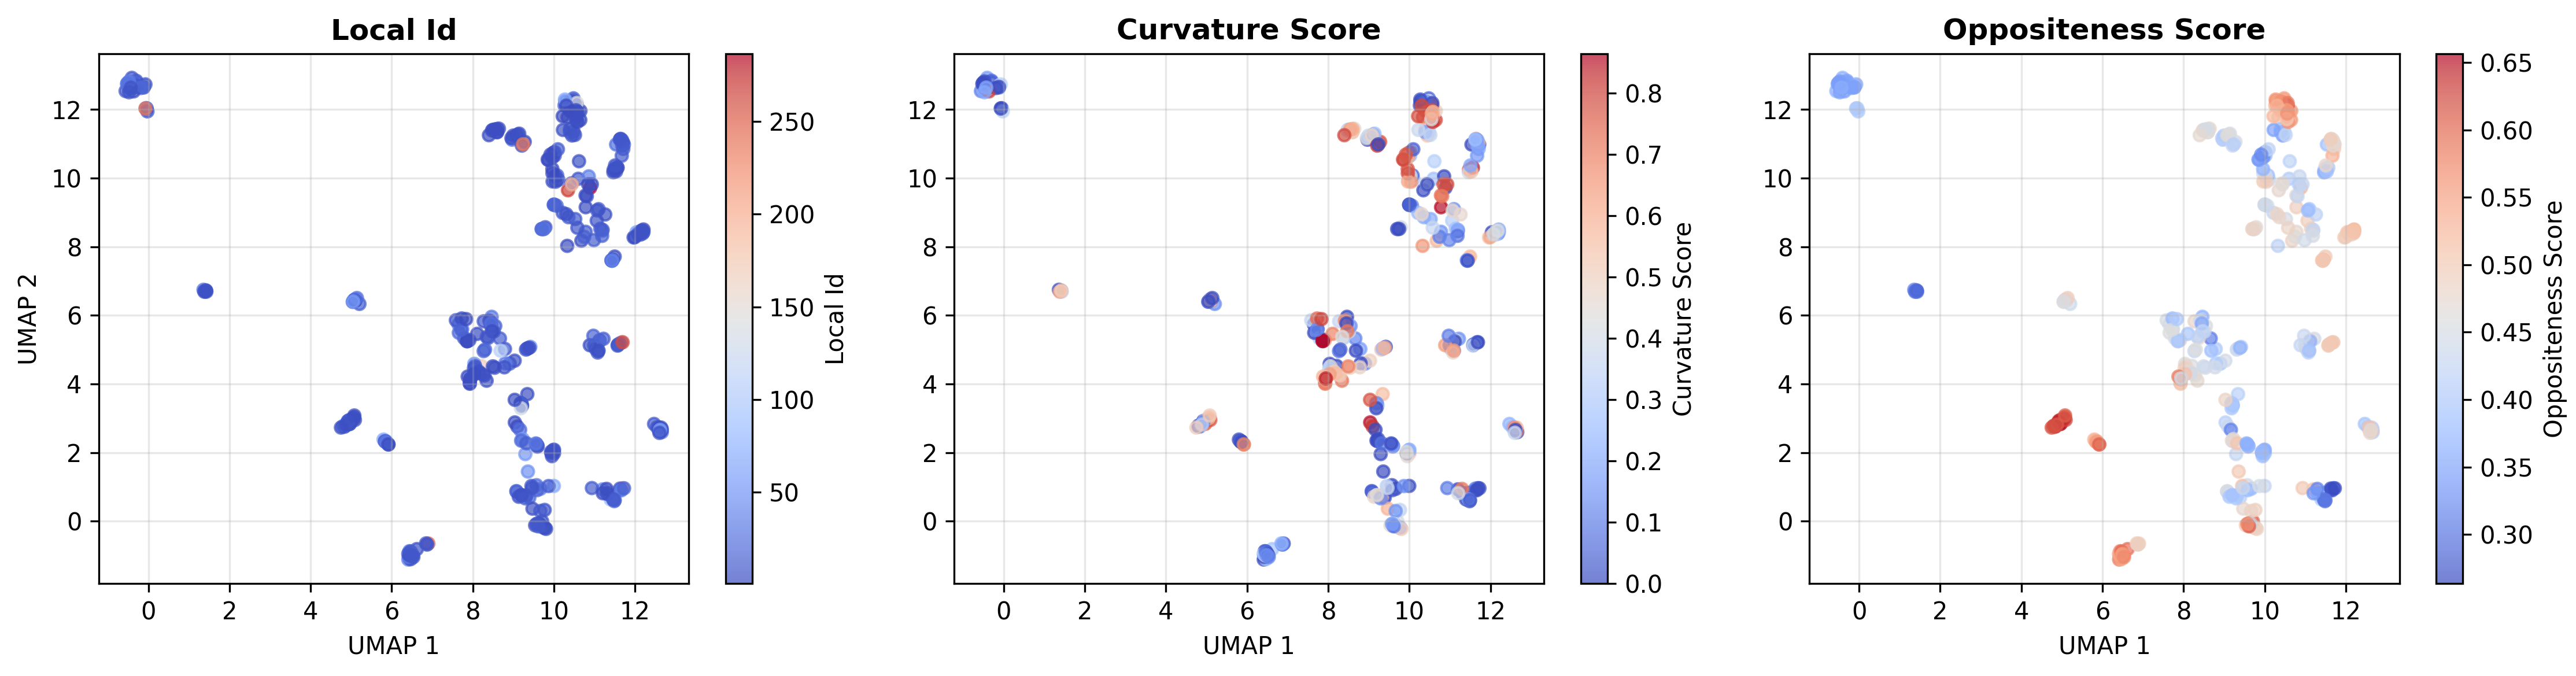
\includegraphics[width=\textwidth]{figures/v3_geometry_heatmaps_umap_a.png}\\[0.5em]
% 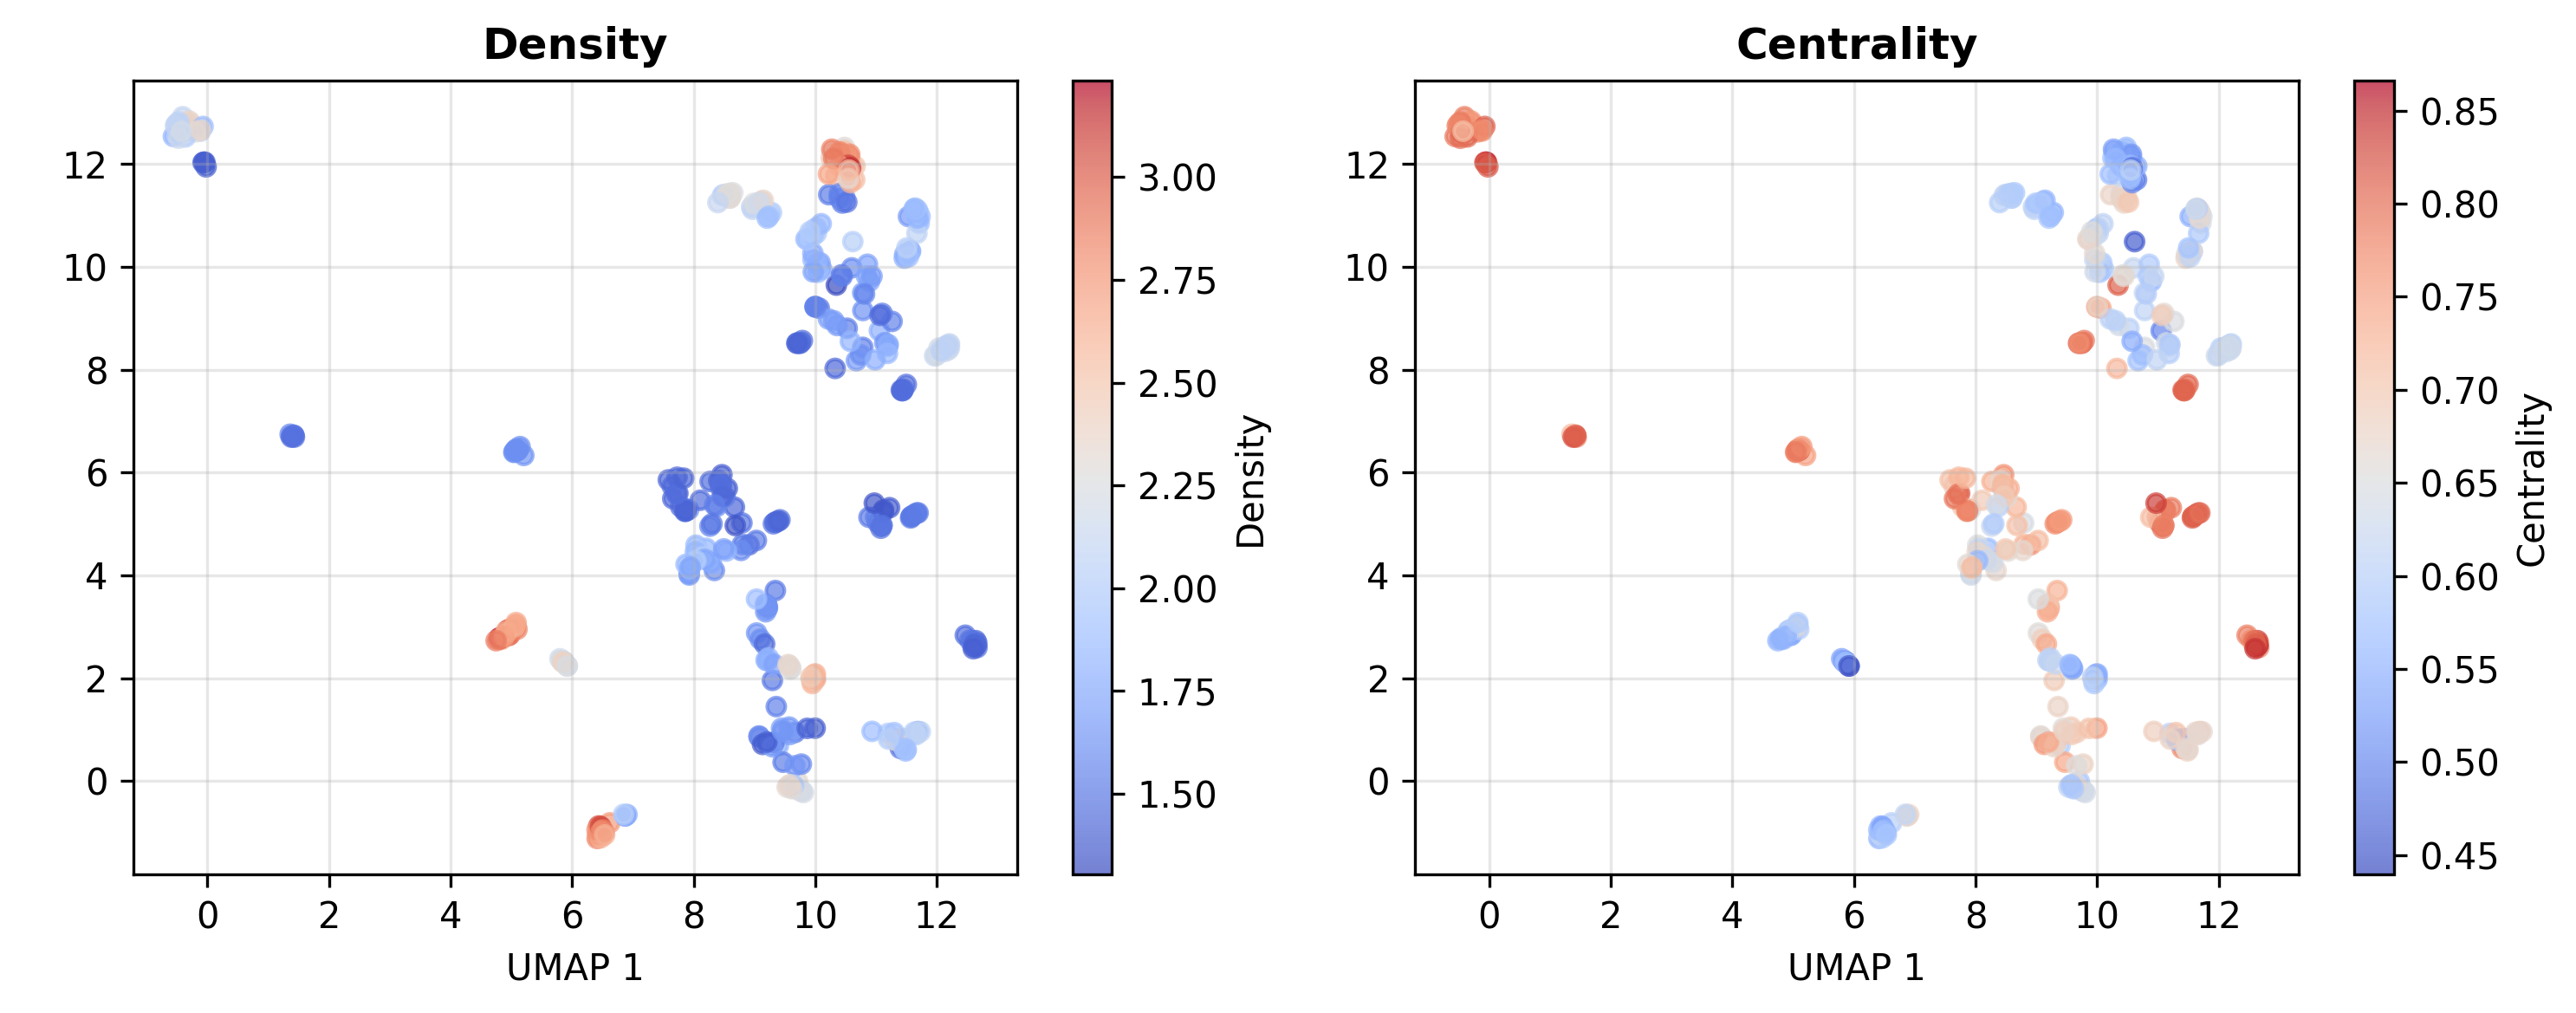
\includegraphics[width=0.67\textwidth]{figures/v3_geometry_heatmaps_umap_b.png}
% \caption{Five geometric features projected onto a UMAP embedding of the 449-prompt initial benchmark. Each point is a prompt; color intensity indicates feature magnitude. Top row: local intrinsic dimension, curvature, and oppositeness. Bottom row: density and centrality. Categories form visually distinct clusters, and feature values covary with cluster membership---foreshadowing the category confound analyzed in Section~\ref{sec:category-confound-preview}. Density and centrality are negatively correlated ($r = -0.51$ on the full 2,879-prompt corpus): sparse regions tend to lie far from the corpus centroid. Oppositeness was computed for the embedding space but was not included in the initial logistic regression.}
% \label{fig:v3-geometry-heatmaps}
% \end{figure}

\subsection{Univariate Feature Differences}
\label{sec:univariate-features}

For each geometric feature, we test whether hallucinated and correct prompts differ using the \emph{Mann-Whitney $U$ test}, a nonparametric test that assumes neither normality nor equal variance. This test is appropriate here given the skewed feature distributions and unequal group sizes. We report the rank-biserial effect size $r = 1 - 2U/(n_1 \cdot n_2)$, where $|r| < 0.1$ is negligible, $0.1$--$0.3$ small, $0.3$--$0.5$ medium, and $> 0.5$ large. We apply Bonferroni correction for multiple comparisons. Partial and refused responses are excluded; only hallucinated (label $= 2$) and correct (label $= 0$) prompts are compared.

Table~\ref{tab:mann-whitney} reports results for all five features. Two show consistent, significant differences across both models: \emph{oppositeness} and \emph{density}. Hallucinated prompts have higher oppositeness and lower density. Both directions are consistent across models.

\begin{table}[ht]
\centering
\small
\begin{tabular}{lcccc}
\toprule
\textbf{Feature} & \textbf{Halluc.\ mean} & \textbf{Correct mean} & $\boldsymbol{p}$ & $\boldsymbol{|r|}$ \\
\midrule
\multicolumn{5}{l}{\textbf{Mixtral 8x7B} ($n_{\text{hall}} = 360$, $n_{\text{correct}} = 2{,}004$)} \\
\addlinespace
\textbf{Oppositeness}    & \textbf{0.513} & \textbf{0.492} & $\boldsymbol{4.5 \times 10^{-11}}$ & \textbf{0.218} \\
\textbf{Density}         & \textbf{2.018} & \textbf{2.085} & $\boldsymbol{1.7 \times 10^{-5}}$  & \textbf{0.142} \\
Centrality      & 0.707 & 0.714 & 0.093                  & 0.056 \\
Curvature       & 0.361 & 0.356 & 0.854                  & 0.006 \\
Local intr.\ dim. & 55.1  & 45.6  & 0.864                  & 0.006 \\
\addlinespace
\midrule
\multicolumn{5}{l}{\textbf{Llama 4 Maverick} ($n_{\text{hall}} = 235$, $n_{\text{correct}} = 2{,}137$)} \\
\addlinespace
\textbf{Oppositeness}    & \textbf{0.526} & \textbf{0.492} & $\boldsymbol{2.5 \times 10^{-20}}$ & \textbf{0.367} \\
\textbf{Centrality}      & \textbf{0.698} & \textbf{0.715} & $\boldsymbol{2.0 \times 10^{-4}}$  & \textbf{0.147} \\
Density         & 2.015 & 2.079 & 0.017                  & 0.095 \\
Curvature       & 0.356 & 0.356 & 0.739                  & 0.013 \\
Local intr.\ dim. & 22.5  & 46.9  & 0.812                  & 0.009 \\
\bottomrule
\end{tabular}
\caption{Mann-Whitney $U$ test results comparing hallucinated versus correct prompts on the expanded benchmark (between-category). Features are sorted by $|r|$ within each model panel. Direction: hallucinated prompts have higher oppositeness and lower density than correct prompts. Bold rows survive Bonferroni correction for 10 comparisons ($\alpha = 0.005$); Llama density ($p = 0.017$) shows the same directional pattern but does not reach the corrected threshold.}
\label{tab:mann-whitney}
\end{table}

Oppositeness shows the largest effect: $|r| = 0.218$ (Mixtral) and $0.367$ (Llama), both highly significant ($p < 10^{-10}$). Density shows a smaller but consistent effect: $|r| = 0.142$ (Mixtral, $p < 10^{-4}$) and $0.095$ (Llama, $p = 0.017$). All significant results survive Bonferroni correction for 10 comparisons ($\alpha = 0.005$), with the exception of Llama's density effect, which shows the same directional pattern as Mixtral but does not reach the corrected threshold.

Centrality is inconsistent across the two models: not significant for Mixtral ($p = 0.093$), but significant for Llama ($p = 0.0002$, $|r| = 0.147$). Hallucinated prompts have lower centrality, meaning they sit closer to the corpus centroid. This is consistent with the initial analysis, where centrality was the dominant predictor ($\beta = -3.62$). This direction likely reflects corpus composition rather than a meaningful geometric signal: the two largest categories (nonexistent and ambiguous, 720 prompts each) sit nearest the corpus centroid (mean centrality $\approx 0.665$ vs.\ $0.710$ corpus-wide) yet have very different hallucination rates (${\sim}30\%$ and ${<}1\%$, respectively), making centrality a weak proxy for category membership. Curvature and local intrinsic dimension show no significant differences for either model (all $p > 0.7$, $|r| < 0.02$), despite curvature and centrality being the two strongest predictors in the initial analysis.

\subsection{Multivariate Prediction}
\label{sec:multivariate-prediction}

To assess combined predictive power, we fit logistic regression models predicting binary hallucination status from standardized geometric features. Models are evaluated via five-fold stratified cross-validation. AUC---the probability that a randomly chosen hallucinated prompt receives a higher predicted risk score than a randomly chosen correct prompt---is $0.645 \pm 0.027$ for Mixtral and $0.726 \pm 0.024$ for Llama (train-set AUC: 0.655 and 0.729, respectively; $\pm$ values are standard deviations across five folds). The small train--CV gaps indicate minimal overfitting.

Table~\ref{tab:logistic-comparison} compares the logistic regression results from the initial analysis with the expanded benchmark analysis. The feature hierarchy has shifted markedly: centrality and curvature, which dominated the initial analysis, are no longer the leading predictors. Instead, oppositeness---which was not measured in the initial analysis---emerges as the strongest predictor for both models, and density rises from non-significant to second. Notably, local intrinsic dimension receives a large standardized coefficient for Llama ($-0.49$) despite showing no univariate signal ($p = 0.81$). This is a hallmark of multicollinearity redistributing weight among correlated predictors. Individual coefficients are unreliable here: oppositeness, density, and centrality share moderate pairwise correlations ($|r| = 0.38$--$0.54$), which redistribute weight among correlated predictors without affecting overall discriminative performance.

\begin{table}[H]
\centering
\small
\begin{tabular}{lcccc}
\toprule
& \multicolumn{2}{c}{\textbf{Initial analysis}} & \multicolumn{2}{c}{\textbf{Expanded benchmark}} \\
\cmidrule(lr){2-3} \cmidrule(lr){4-5}
\textbf{Feature} & $\beta$ & $p$ & Mixtral $\beta_z$ & Llama $\beta_z$ \\
\midrule
Centrality      & $-3.62$ & ${<}0.001$ & $-0.03$ & $-0.13$ \\
Curvature       & $-1.21$ & ${<}0.001$ & $-0.02$ & $-0.09$ \\
Density         & $-0.15$ & $0.482$    & $-0.45$ & $-0.66$ \\
Local intr.\ dim. & $\approx 0$ & $0.983$ & $+0.01$ & $-0.49$ \\
Oppositeness    & ---     & ---        & $+0.55$ & $+0.85$ \\
\midrule
\textbf{AUC}    & \multicolumn{2}{c}{0.86 (train)} & 0.645 (CV) & 0.726 (CV) \\
\bottomrule
\end{tabular}
\caption{Logistic regression coefficients for predicting hallucination from geometric features. Initial analysis: unstandardized coefficients ($\beta$) from pooled 10-model analysis on 368 prompts across four categories (4 features, balanced class weights, train-set AUC). Expanded benchmark: standardized coefficients ($\beta_z$) from per-model analysis on 2,430 prompts (5 features, no class reweighting, five-fold cross-validated AUC). Oppositeness was not measured in the initial analysis. The dominant predictors shift from centrality and curvature to oppositeness and density.}
\label{tab:logistic-comparison}
\end{table}

The cross-validated AUC of 0.64--0.73 represents a substantial drop from the initial analysis's train-set AUC of 0.86. The drop is not primarily overfitting---the small train-CV gap rules that out---but rather category structure absorbing most of the signal. The next section formalizes this decomposition.

\subsection{The Role of Category Structure}
\label{sec:category-confound-preview}

The results above are real: hallucinated prompts genuinely occupy geometrically distinct regions of embedding space. But they may be partly circular. Our seven categories span a deliberate difficulty gradient (Table~\ref{tab:category-rates}): the highest-hallucination category exceeds 40\% (Mixtral), while the lowest falls below 1\%. If these categories themselves also differ in their geometric properties---and they do, as categories with higher hallucination rates tend toward lower density and higher oppositeness---then a classifier could achieve decent AUC by implicitly detecting category membership rather than fine-grained geometric structure within a category.

\begin{figure}[H]
\centering
\includegraphics[width=\textwidth]{figures/v5_category_umap_combined.png}
\caption{UMAP (Uniform Manifold Approximation and Projection \citep{mcinnes2018umap}) projection of the 2,430-prompt expanded benchmark, colored by category. Categories form distinct clusters in the embedding space. Hallucination rates (in parentheses in the legend, computed from Mixtral baseline labels) vary dramatically across clusters: nonexistent (29.5\%) and plausible fake (43.5\%) versus ambiguous (0.7\%) and edge factual (3.1\%). A classifier need only detect which cluster a prompt falls in---without learning any within-category geometric structure---to achieve substantial predictive power.}
\label{fig:category-umap}
\end{figure}

\section{Decomposing Category vs.\ Geometric Signal}
\label{sec:decomposition}

To quantify how much of the geometric signal reflects category structure rather than within-category variation, we compare three nested logistic regression models that progressively isolate geometry's contribution.

\paragraph{Three-model decomposition.} We fit three logistic regression models predicting binary hallucination status (hallucinated vs.\ all non-hallucinated responses, including partial and refused):

\begin{enumerate}
    \item \textbf{Geometry-only}: The five geometric features, $z$-scored to zero mean and unit variance. This is the model reported in Section~\ref{sec:multivariate-prediction}.
    \item \textbf{Category-only}: Six indicator variables from one-hot encoding of the seven categories (one dropped to avoid perfect collinearity), with no geometric information. This baseline captures category-level difficulty alone.
    \item \textbf{Category + Geometry}: All five geometric features plus six category indicators (11 predictors total). The AUC improvement from Model~2 to Model~3 isolates geometry's marginal contribution beyond category membership.
\end{enumerate}

\noindent All three models use five-fold stratified cross-validation with identical fold assignments. Table~\ref{tab:decomposition} reports the results.

\begin{table}[ht]
\centering
\begin{tabular}{lcc}
\toprule
\textbf{Model} & \textbf{Mixtral CV AUC} & \textbf{Llama CV AUC} \\
\midrule
Geometry-only (5 features)          & 0.645 & 0.726 \\
Category-only (6 indicators)        & 0.782 & 0.773 \\
Category + Geometry (11 features)   & 0.800 & 0.814 \\
\midrule
Geometry increment                  & $+$0.018 & $+$0.041 \\
\bottomrule
\end{tabular}
\caption{Decomposing predictive signal: five-fold stratified cross-validated (CV) AUC for predicting binary hallucination status on the expanded benchmark. Geometry features are $z$-scored; category indicators use one-hot encoding with one category dropped. The geometry increment is the difference between the category+geometry and category-only AUCs.}
\label{tab:decomposition}
\end{table}

Category membership alone is a strong predictor, achieving AUC 0.782 (Mixtral) and 0.773 (Llama), which is not surprising given the deliberate difficulty gradient built into our benchmark design. The geometry-only model falls well below the category-only baseline for Mixtral (0.645 vs.\ 0.782) and moderately below for Llama (0.726 vs.\ 0.773), indicating that the five geometric features, operating without category labels, are less informative than knowing which category a prompt belongs to. Adding geometry to category yields an increment of $+$0.018 for Mixtral and $+$0.041 for Llama. Most of the geometric signal identified in Section~\ref{sec:between-category}---the lower density and higher oppositeness of hallucinated prompts---tracks category membership rather than within-category variation. The larger Llama increment is consistent with Llama's stronger between-category oppositeness effect ($|r| = 0.367$ vs.\ $0.218$ for Mixtral; Table~\ref{tab:mann-whitney}), suggesting that geometry captures more model-specific signal for Llama beyond what category labels provide.

\paragraph{Why this is not a negative result.} These results should not be dismissed as purely circular. The embedding space independently recovers a difficulty gradient that aligns with our human-designed taxonomy---categories were defined semantically, not geometrically, yet a geometry-only classifier achieves AUC 0.65--0.73 without category labels. The nonzero increment means that, conditional on category membership, prompts with different geometry carry different hallucination risk. And the aggregate increment understates within-category effects by construction. Pooling $+$0.02--0.04 AUC over seven categories---four of which have hallucination rates below 10\%---could mask larger effects within high-hallucination categories.

\paragraph{Reconciling with the initial analysis.} The initial AUC of 0.86 drops to 0.645--0.726 under cross-validation. Three methodological differences account for this: (a)~train-set evaluation without cross-validation; (b)~pooling across 10 models, conflating model-level tendencies with prompt-level geometry; and (c)~no separation of category-level from within-category signal. The decomposition above (Table~\ref{tab:decomposition}) shows that category alone achieves AUC 0.77--0.78, absorbing most of the initial analysis's discriminative power. The initial result correctly detected that geometric features carry hallucination information; the expanded analysis decomposes this into a dominant category-level component and a more modest within-category component.

% \begin{figure}[H]
% \centering
% 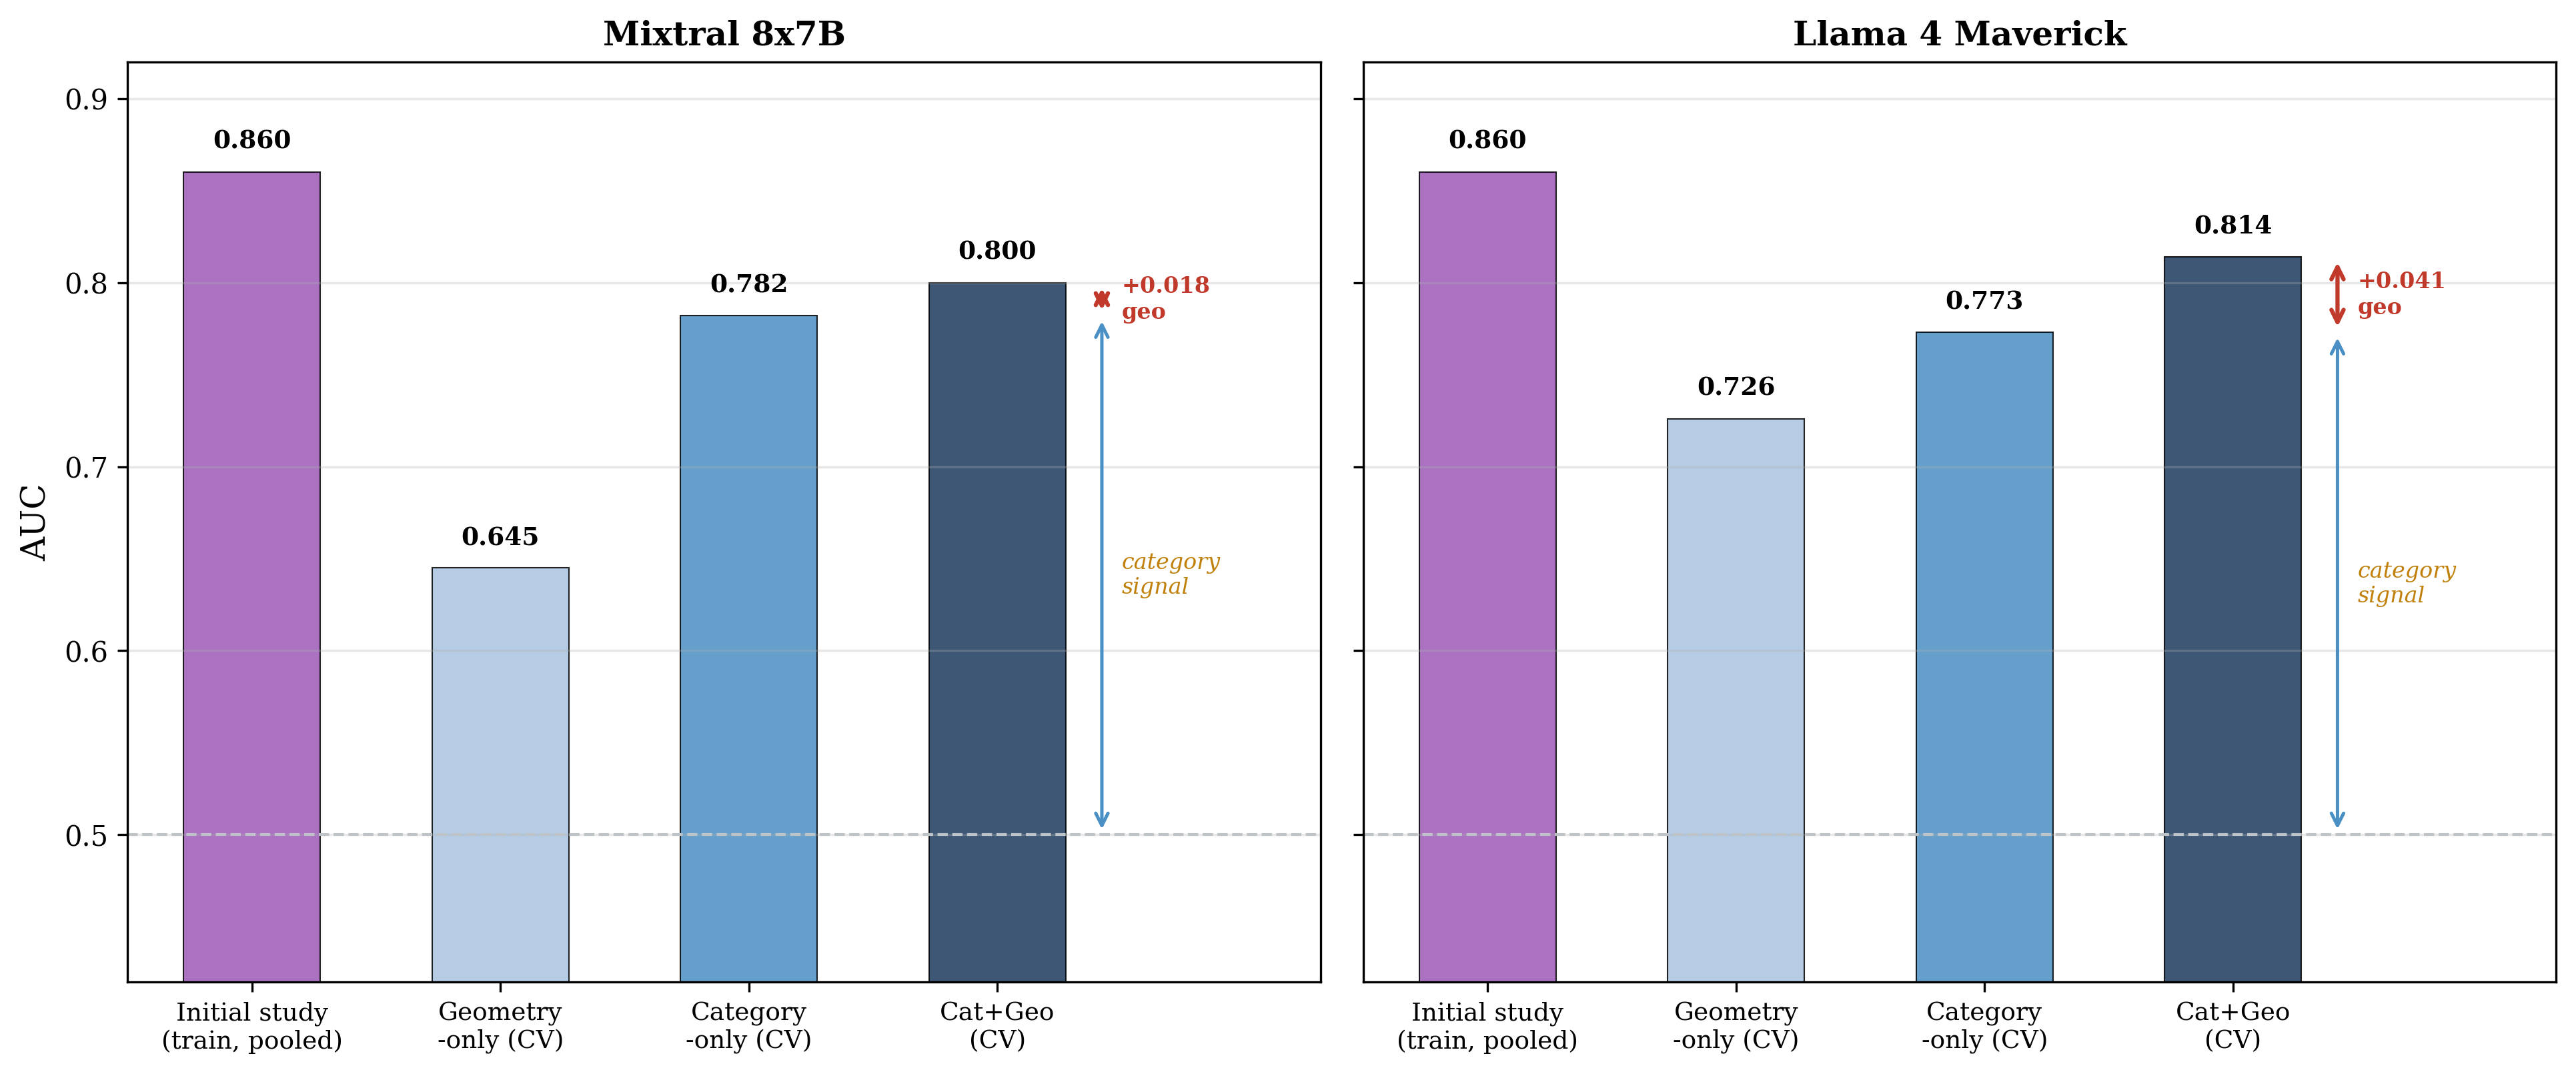
\includegraphics[width=\textwidth]{figures/ch5_signal_decomposition.png}
% \caption{Reconciling the initial analysis with the expanded analysis. The initial analysis's train-set AUC of 0.86 (purple) substantially exceeds the cross-validated, per-model AUCs on the expanded benchmark. The decomposition reveals that category membership alone (orange) accounts for most predictive power (AUC 0.77--0.78); geometry adds a modest increment (green annotations on the right). The gap between the initial analysis and the expanded analysis reflects methodological refinements: cross-validation, per-model analysis, and category-level controls.}
% \label{fig:signal-decomposition}
% \end{figure}

\paragraph{The critical test.} The decomposition shows that most aggregate predictive power overlaps with category structure. But the nonzero geometry increment, together with the fact that categories were defined semantically rather than geometrically, suggests genuine within-category signal. The critical test is whether geometric features predict hallucination \emph{within} individual categories, controlling entirely for category-level confounds. If, among hundreds of prompts that share the same category, the same prompt structure, and the same type of knowledge failure, the ones in sparser embedding neighborhoods hallucinate more, that signal cannot be attributed to category membership.

Figure~\ref{fig:within-cat-auc-preview} previews where this signal exists. Within-category logistic regression AUC varies dramatically: the nonexistent category (the largest, with the most hallucinations) shows the strongest within-category geometric signal for both models, while categories with few hallucinations fall at or below chance. Section~\ref{sec:within-category} analyzes these patterns in detail.

\begin{figure}[H]
\centering
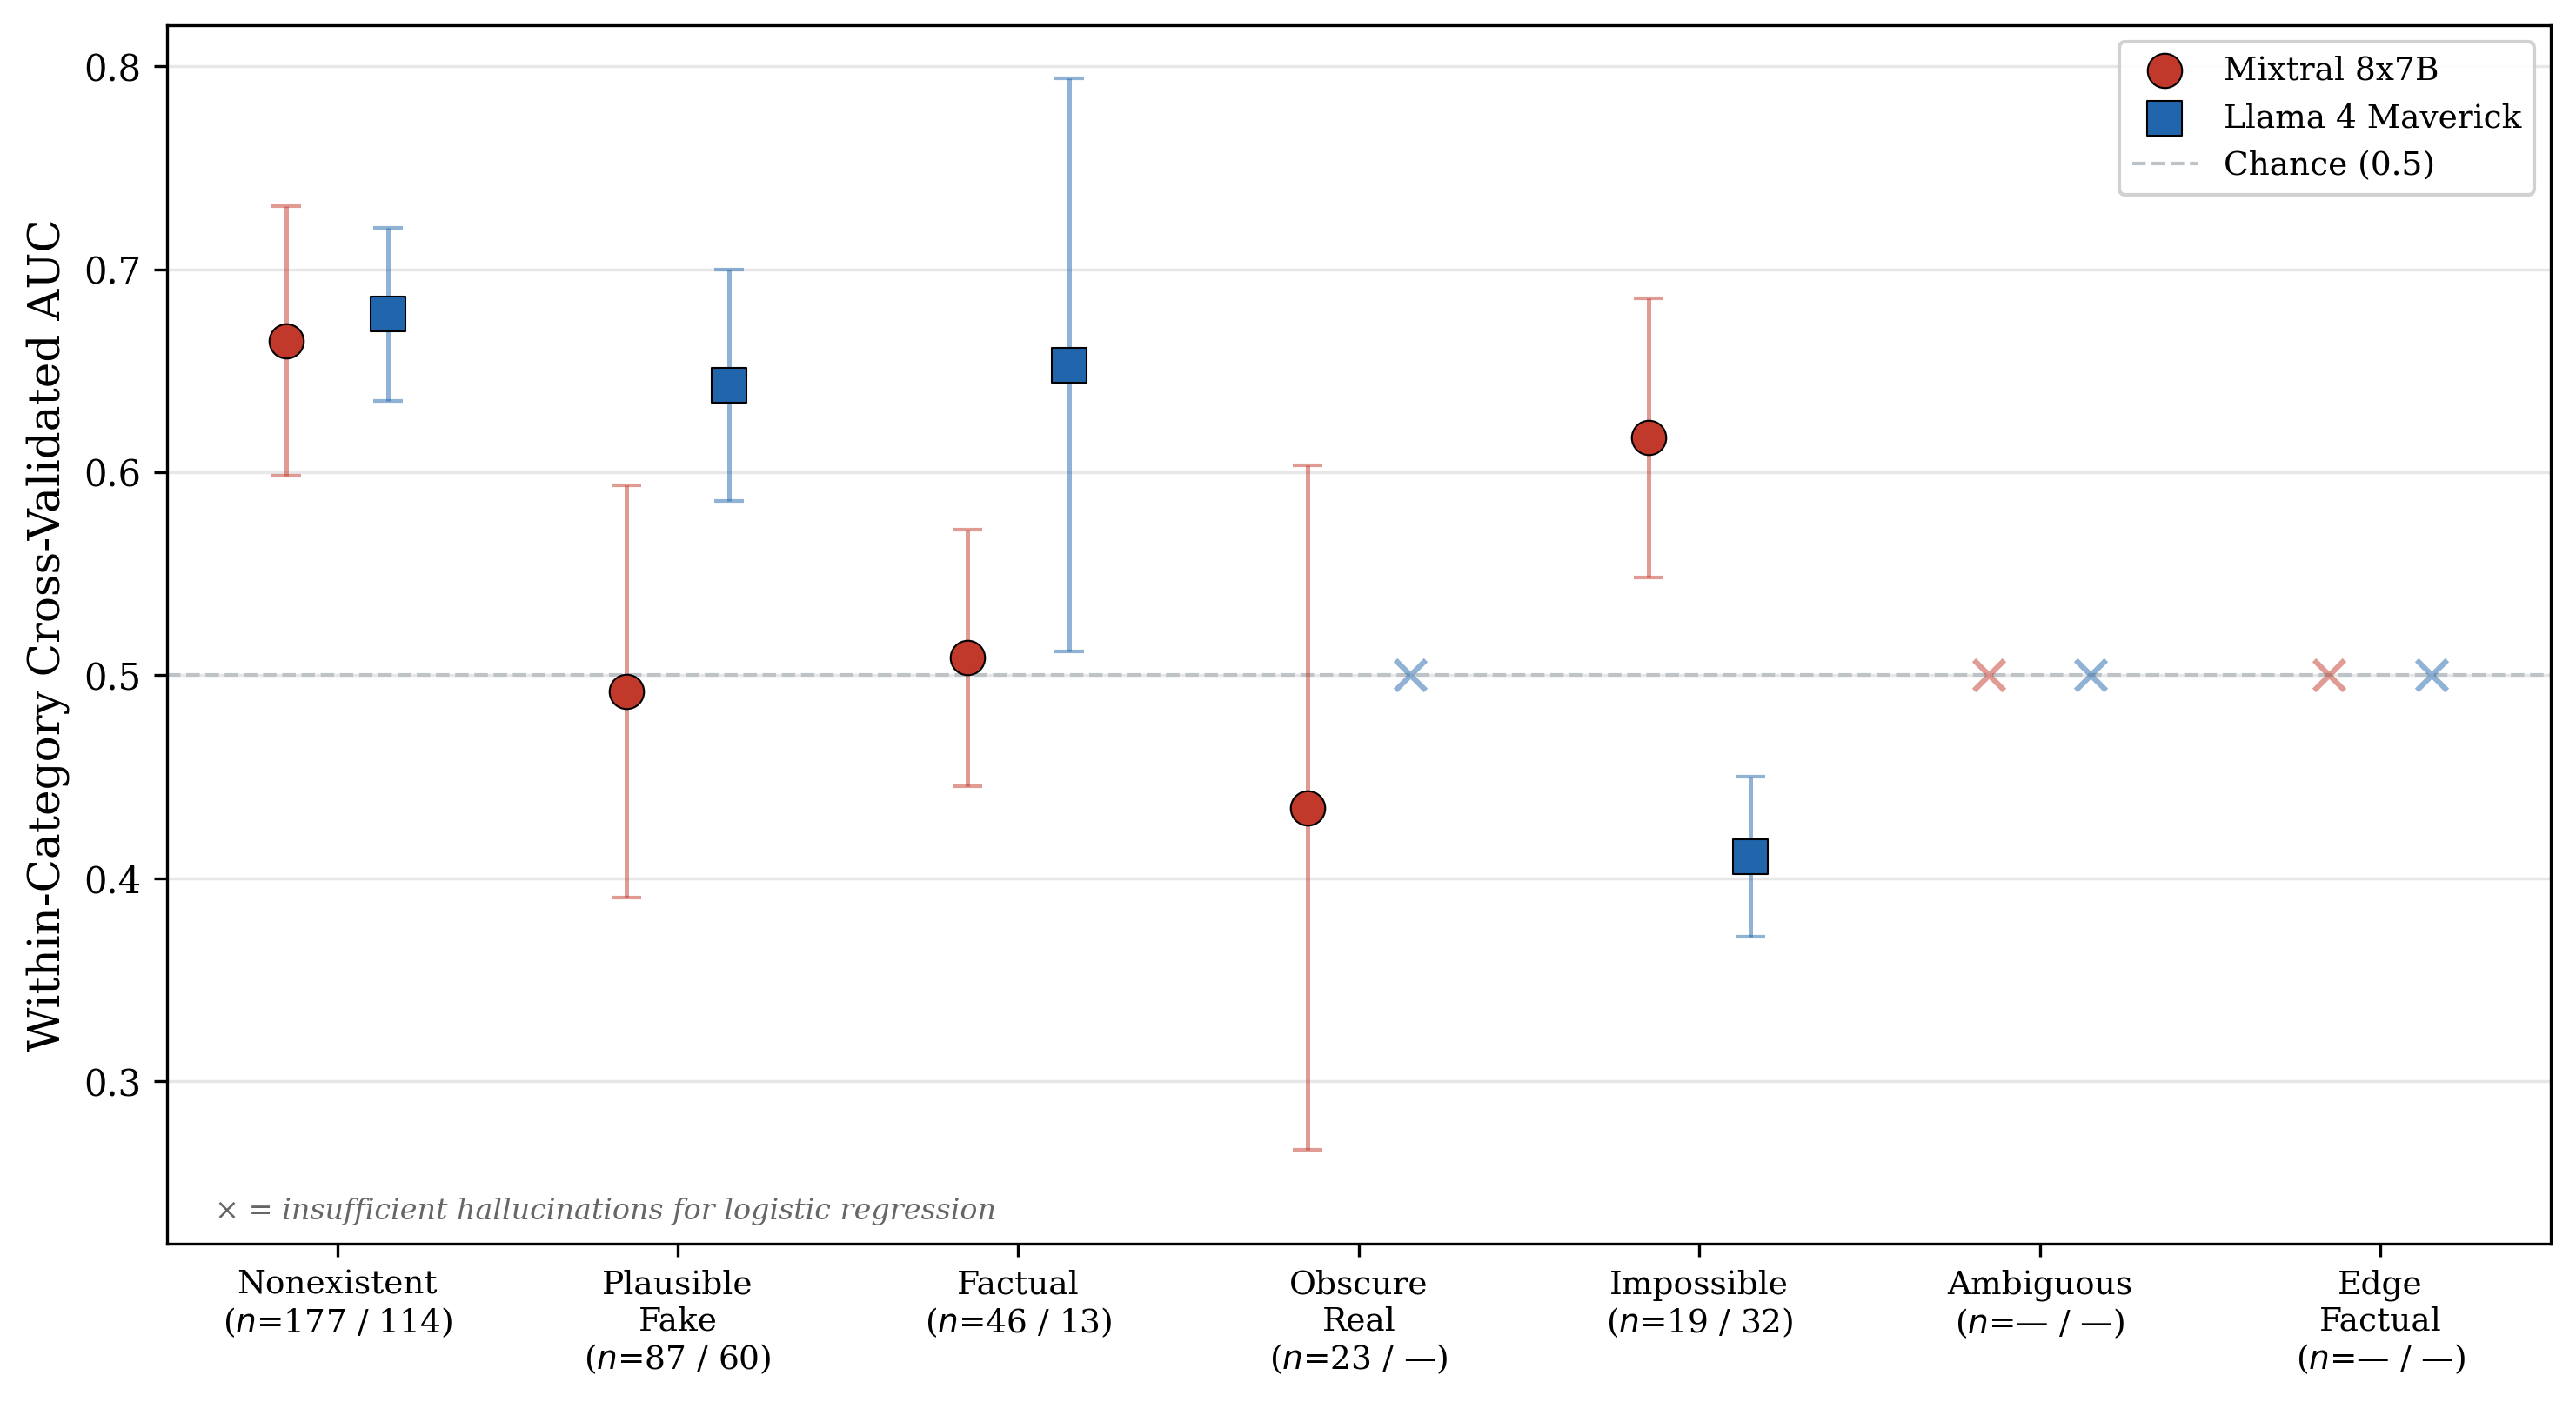
\includegraphics[width=\textwidth]{figures/ch5_within_category_auc_dots.png}
\caption{Within-category cross-validated AUC for predicting hallucination from geometric features alone, by category. Error bars show standard deviation across five folds; $n$ labels indicate the number of hallucinated prompts for Mixtral / Llama, respectively (dashes indicate insufficient counts for logistic regression). The nonexistent category shows the strongest geometric signal for both models (AUC $\approx 0.67$). Categories with fewer hallucinations have wide error bars or fall near chance. Crosses indicate categories excluded due to insufficient hallucination counts.}
\label{fig:within-cat-auc-preview}
\end{figure}

\section{Within-Category Geometric Analysis}
\label{sec:within-category}

The decomposition showed that a nonzero geometry increment persists after controlling for category membership, but the aggregate effect is modest. The critical test is whether geometric features predict hallucination \emph{within} individual categories, where category membership is held constant and cannot inflate prediction. We apply the same Mann-Whitney $U$ tests and logistic regression methodology from the between-category analysis, now separately within each category.

\subsection{Within-Category Predictive Power}
\label{sec:within-cat-auc}

Table~\ref{tab:within-category-auc} reports the within-category cross-validated AUC for predicting hallucination from the five geometric features. Categories with too few hallucinated prompts for reliable five-fold stratified cross-validation are excluded (indicated by dashes). Figure~\ref{fig:within-cat-auc-preview} visualizes these results.

\begin{table}[ht]
\centering
\small
\begin{tabular}{lrcrc}
\toprule
& \multicolumn{2}{c}{\textbf{Mixtral}} & \multicolumn{2}{c}{\textbf{Llama}} \\
\cmidrule(lr){2-3} \cmidrule(lr){4-5}
\textbf{Category} & $n_{\text{hall}}$ & \textbf{AUC $\pm$ SD} & $n_{\text{hall}}$ & \textbf{AUC $\pm$ SD} \\
\midrule
Nonexistent         & 177 & $\mathbf{0.665 \pm 0.066}$ & 114 & $\mathbf{0.678 \pm 0.042}$ \\
Plausible fake      &  87 & $0.492 \pm 0.102$          &  60 & $0.643 \pm 0.057$ \\
Factual             &  46 & $0.509 \pm 0.063$          &  13 & $0.653 \pm 0.141$ \\
Impossible          &  19 & $0.617 \pm 0.069$          &  32 & $0.411 \pm 0.039$ \\
Obscure real        &  23 & $0.435 \pm 0.169$          &   6 & --- \\
Ambiguous           &   4 & ---                        &   9 & --- \\
Edge factual        &   4 & ---                        &   1 & --- \\
\bottomrule
\end{tabular}
\caption{Within-category AUC ($\pm$ standard deviation across five cross-validation folds) for predicting hallucination from five geometric features. Dashes indicate categories excluded due to insufficient hallucination counts for five-fold stratified cross-validation. Bold indicates the category with AUC reliably above chance for both models. Categories are sorted by decreasing sample size.}
\label{tab:within-category-auc}
\end{table}

The results are strikingly heterogeneous. The nonexistent category---the largest (600 prompts) and the one with the most hallucinations---shows the strongest and most consistent within-category geometric signal: AUC $0.665 \pm 0.066$ (Mixtral, $n_{\text{hall}} = 177$) and $0.678 \pm 0.042$ (Llama, $n_{\text{hall}} = 114$). The small standard deviations indicate stable performance across folds.

Other categories show weaker or inconsistent signal. Llama's plausible fake category reaches AUC $0.643$, but Mixtral falls to chance ($0.492$) on the same category. Llama's factual category shows AUC $0.653$, but with only 13 hallucinated prompts and a standard deviation of $0.141$, this estimate is unreliable. Mixtral's impossible category shows moderate signal ($0.617$, $n_{\text{hall}} = 19$), but Llama's impossible category falls below chance ($0.411$). Categories with hallucination rates below 3\%---ambiguous and edge factual---lack sufficient positive cases for within-category analysis entirely.

The pattern is clear: within-category geometric prediction works where there are enough hallucinations to predict. The nonexistent category, with 177 and 114 hallucinated prompts for the two models, provides the statistical power that other categories lack. The absence of signal in smaller categories likely reflects insufficient power rather than a genuine null: even the enrichment of nominally significant results across all categories (11 of 55 tests reach $p < 0.05$, versus ${\sim}2.8$ expected by chance) suggests signal beyond nonexistent.

\subsection{Density as the Consistent Within-Category Predictor}
\label{sec:within-cat-density}

To identify which features drive the within-category signal, we examine Mann-Whitney $U$ results within the nonexistent category, as it is the only category with sufficient power for robust inference across all five features and both models. Table~\ref{tab:within-cat-nonexistent} reports the results.

\begin{table}[ht]
\centering
\small
\begin{tabular}{lcccc}
\toprule
\textbf{Feature} & \textbf{Halluc.\ mean} & \textbf{Correct mean} & $\boldsymbol{p}$ & $\boldsymbol{|r|}$ \\
\midrule
\multicolumn{5}{l}{\textbf{Mixtral 8x7B} ($n_{\text{hall}} = 177$, $n_{\text{correct}} = 419$)} \\
\addlinespace
\textbf{Density}         & \textbf{2.165} & \textbf{2.316} & $\boldsymbol{5.7 \times 10^{-7}}$ & \textbf{0.259} \\
\textbf{Oppositeness}    & \textbf{0.532} & \textbf{0.520} & $\boldsymbol{4.6 \times 10^{-3}}$ & \textbf{0.147} \\
Centrality      & 0.680 & 0.665 & $0.011$               & 0.132 \\
Local intr.\ dim. & 23.4  & 37.5  & $0.612$               & 0.026 \\
Curvature       & 0.352 & 0.355 & $0.974$               & 0.002 \\
\addlinespace
\midrule
\multicolumn{5}{l}{\textbf{Llama 4 Maverick} ($n_{\text{hall}} = 114$, $n_{\text{correct}} = 484$)} \\
\addlinespace
\textbf{Density}         & \textbf{2.132} & \textbf{2.303} & $\boldsymbol{3.4 \times 10^{-5}}$ & \textbf{0.249} \\
Centrality      & 0.680 & 0.668 & $0.029$               & 0.131 \\
Oppositeness    & 0.533 & 0.522 & $0.037$               & 0.126 \\
Local intr.\ dim. & 27.7  & 34.5  & $0.075$               & 0.107 \\
Curvature       & 0.313 & 0.364 & $0.085$               & 0.103 \\
\bottomrule
\end{tabular}
\caption{Within-category Mann-Whitney $U$ test results for the nonexistent category (600 prompts). Features sorted by $|r|$ within each model. Hallucinated prompts occupy sparser neighborhoods (lower density) and show higher oppositeness. Bold rows survive Bonferroni correction for 10 comparisons ($\alpha = 0.005$). Density also survives the study-wide correction across all within-category comparisons ($\alpha = 0.05/70 = 0.0007$).}
\label{tab:within-cat-nonexistent}
\end{table}

\begin{figure}[ht]
\centering
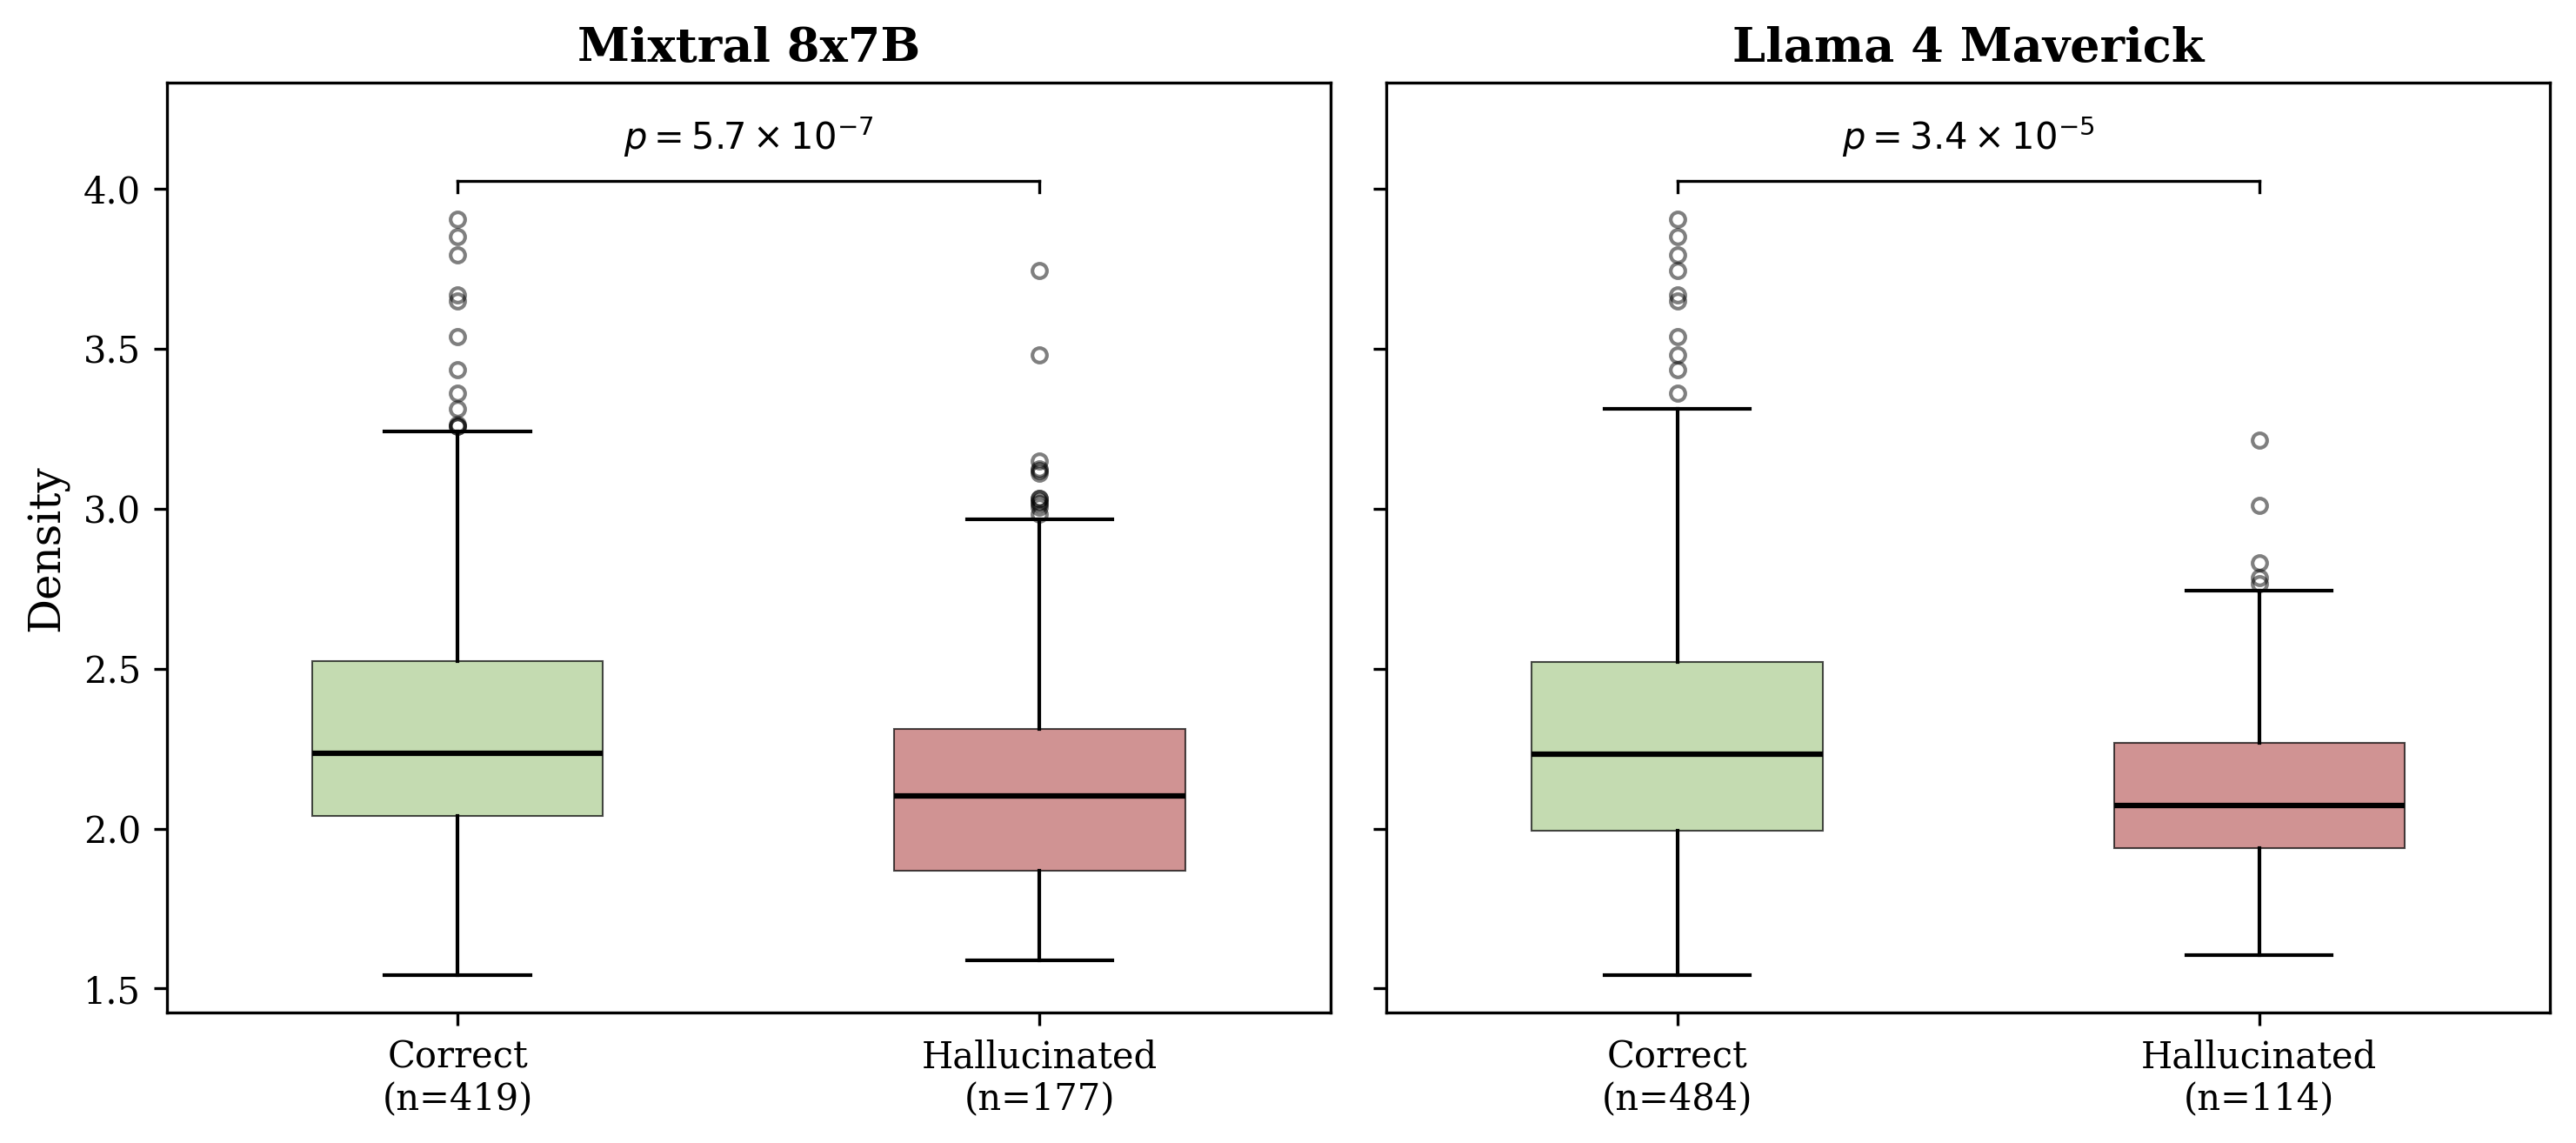
\includegraphics[width=0.95\textwidth]{figures/ch5_within_category_density_nonexistent.png}
\caption{Density distributions for hallucinated versus correctly answered prompts within the nonexistent category. Hallucinated prompts occupy sparser embedding neighborhoods (lower density) for both models. Mann-Whitney $U$ $p$-values survive Bonferroni correction ($\alpha = 0.005$). Box plots show median, interquartile range, and $1.5\times$ IQR whiskers; circles denote outliers.}
\label{fig:within-cat-density}
\end{figure}

Density is the dominant within-category predictor for both models (Figure~\ref{fig:within-cat-density}). Among the 600 nonexistent prompts, those that trigger hallucination have substantially lower density---meaning their embedding neighborhoods are sparser---than those answered correctly. The effect sizes ($|r| = 0.259$ and $0.249$) are small to medium by conventional thresholds and are the largest for any feature in either model. Both $p$-values survive Bonferroni correction for 10 comparisons ($\alpha = 0.005$), and Mixtral's density result ($p = 5.7 \times 10^{-7}$) survives even the most conservative study-wide correction across all within-category tests.

The direction is consistent with the between-category finding (Table~\ref{tab:mann-whitney}): sparser embedding neighborhoods predict hallucination at both levels of analysis.

Oppositeness and centrality show suggestive effects ($p < 0.05$, uncorrected), but are not consistently significant across both models after correction. Mixtral's within-category oppositeness narrowly survives Bonferroni correction ($p = 0.0046$ vs.\ $\alpha = 0.005$); Llama's does not ($p = 0.037$). Centrality shows nominally significant effects for both models ($p = 0.011$ and $0.029$), but the within-category direction \emph{reverses} from the between-category analysis: within the nonexistent category, hallucinated prompts have \emph{higher} centrality (farther from the corpus centroid), whereas between categories, hallucinated prompts have lower centrality (closer to the corpus centroid). This reversal is an instance of Simpson's paradox---a phenomenon in which a trend that appears in aggregated data reverses when the data are partitioned into subgroups. The reversal is consistent with two different forces operating at different scales: category composition drives the aggregate direction (high-hallucination categories happen to sit closer to the corpus centroid), while within-category isolation may drive the local signal. That the within-category direction aligns with the density finding---peripheral, less-connected prompts hallucinate more---suggests both features capture aspects of the same underlying structure. Neither within-category centrality effect survives Bonferroni correction, so this interpretation remains tentative.

Curvature and local intrinsic dimension show no within-category signal (all $p > 0.07$), consistent with their null results in the between-category analysis.

\paragraph{Signal in other categories.} Beyond the nonexistent category, two results merit brief mention. Llama's borderline plausible fake category shows a significant oppositeness effect ($p = 0.003$, $|r| = 0.268$, $n_{\text{hall}} = 60$), consistent with this category's moderate within-category AUC of 0.643 for Llama. Mixtral's impossible category shows a density effect ($p = 0.014$, $|r| = 0.345$, $n_{\text{hall}} = 19$) with the same direction as the nonexistent finding---sparser neighborhoods predict hallucination. Neither result survives correction for the full set of within-category comparisons.

\paragraph{Interpretation.} The within-category density finding is the central result of this chapter. It establishes that, among hundreds of prompts that share the same category label, the same type of knowledge failure, and similar prompt structures, the ones whose embeddings fall in sparser neighborhoods of the embedding space are more likely to trigger hallucination. This signal cannot be attributed to category membership.

Why density carries this signal---and what it means mechanistically---is discussed in Section~\ref{sec:ch5-discussion}. Section~\ref{sec:feature-synthesis} first synthesizes the feature hierarchy across all analyses in this chapter.

\section{Feature Synthesis}
\label{sec:feature-synthesis}

The preceding sections tested five geometric features at three levels: univariate between-category, multivariate with and without category controls, and univariate within-category. The feature hierarchy reversed between the initial and expanded analyses. This section synthesizes the evidence into a per-feature assessment.

\subsection{Per-Feature Assessment}

Table~\ref{tab:feature-synthesis} summarizes the evidence across all three levels of analysis.

\begin{table}[ht]
\centering
\small
\begin{tabular}{@{}p{2.0cm}p{2.5cm}p{3.2cm}p{3.2cm}p{2.8cm}@{}}
\toprule
\textbf{Feature} & \textbf{Initial analysis} \newline (368 prompts) & \textbf{Between-cat.} \newline (expanded, 2{,}430; M/L) & \textbf{Within-cat.} \newline (nonexistent, 600; M/L) & \textbf{Assessment} \\
\midrule
Oppositeness & Not measured & Strongest: $|r|{=}0.218$/$0.367$, $p < 10^{-10}$ & $p{=}0.0046$/$0.037$; plaus.\ fake (Llama): $p{=}0.003$ & Strong between-cat.; mixed within-cat. \\
\addlinespace
\textbf{Density} & Non-sig.\ ($\beta{=}{-}0.15$, $p{=}0.48$) & Second: $|r|{=}0.142$/$0.095$, $p < 10^{-4}$/$0.017$ & $p{=}5.7{\times}10^{-7}$ / \newline $p{=}3.4{\times}10^{-5}$ (\textbf{Bonf.}) & \textbf{Survives all controls} \\
\addlinespace
Centrality & Strongest ($\beta{=}{-}3.62$, $p{<}0.001$) & Weak: $|r|{=}0.056$/$0.147$, $p{=}0.093$/$0.0002$ & Direction reverses; $p{=}0.011$/$0.029$ (uncorr.) & Downgraded --- was proxying for category \\
\addlinespace
Curvature & Second ($\beta{=}{-}1.21$, $p{<}0.001$) & Null: $|r|{<}0.02$, $p > 0.7$ & Null: $p > 0.07$ & Downgraded --- not robust \\
\addlinespace
Local intr.\ dim. & Null ($\beta{\approx}0$, $p{=}0.98$) & Null: $|r|{<}0.01$, $p > 0.8$ & Null: $p > 0.07$ & Confirmed null \\
\bottomrule
\end{tabular}
\caption{Feature synthesis across three levels of analysis. Initial analysis coefficients ($\beta$) are unstandardized from pooled 10-model logistic regression on 368 prompts (four categories); between-category and within-category results report Mann-Whitney rank-biserial $|r|$ and $p$-values (Mixtral/Llama). ``Bonf.'' indicates survival of Bonferroni correction across all 70 possible within-category comparisons (7 categories $\times$ 5 features $\times$ 2 models; $\alpha = 0.05/70 = 0.0007$), including categories excluded from testing due to insufficient hallucination counts. Oppositeness was not measured in the initial analysis (only four features: centrality, curvature, density, local intrinsic dimension).}
\label{tab:feature-synthesis}
\end{table}

\subsection{Why Centrality and Curvature Were Downgraded}
\label{sec:centrality-curvature}

Centrality dominated the initial analysis ($\beta = -3.62$) because high-hallucination categories (nonexistent, plausible fake) happen to cluster closer to the corpus centroid than low-hallucination categories. It was proxying for ``which category is this?'' rather than fine-grained geometry. The Simpson's paradox in Section~\ref{sec:within-cat-density} confirms this: between categories, hallucinated prompts have lower centrality, but within the nonexistent category the direction reverses (hallucinated prompts sit farther from the centroid, $p = 0.011$/$0.029$, uncorrected). Curvature follows a similar pattern: significant in the initial analysis ($\beta = -1.21$) but null at both levels in the expanded analysis (all $|r| < 0.02$ between categories, all $p > 0.07$ within). Both features' initial significance reflected category-correlated variance amplified by balanced class weighting and 10-model pooling.

\subsection{Density as the Robust Signal}
\label{sec:density-robust}

Density was non-significant in the initial analysis ($\beta = -0.15$, $p = 0.48$), but it is the most robust predictor in the expanded analysis: significant between categories ($p < 10^{-4}$ for Mixtral), significant within the nonexistent category for both models ($p = 5.7 \times 10^{-7}$ and $3.4 \times 10^{-5}$---the only results surviving study-wide Bonferroni correction), and consistent in direction at both levels. Its initial non-significance reflects centrality absorbing overlapping variance ($r = -0.509$ between the two features) in the smaller dataset.
\subsection{Oppositeness: Between Category but Not Within}
\label{sec:oppositeness-assessment}

Oppositeness is the strongest between-category discriminator ($|r| = 0.218$ for Mixtral, $0.367$ for Llama), but its within-category evidence is mixed. Within the nonexistent category, Mixtral shows a borderline effect ($p = 0.0046$, just below the within-table Bonferroni threshold of $0.005$) while Llama's effect is weaker ($p = 0.037$, not surviving correction). Llama's plausible fake category shows a notable within-category oppositeness effect ($p = 0.003$, $|r| = 0.268$), but this does not replicate in Mixtral's plausible fake results ($p = 0.264$).

Whether oppositeness captures genuine within-category signal or residual between-category structure remains an open question. Unlike density, it does not show consistent within-category significance across both models for any single category. We note that oppositeness was not available in the initial analysis---it was computed from corpus-level PCA and introduced only for the expanded benchmark---so no longitudinal comparison is possible.

\subsection{Feature Correlations and Multicollinearity}
\label{sec:feature-correlations}

The five features are not independent. Moderate pairwise correlations exist among oppositeness, centrality, and density ($|r| = 0.38$--$0.54$); all other pairs are weak ($|r| < 0.15$). This explains the instability of logistic regression coefficients (e.g., Llama's anomalous local intrinsic dimension coefficient of $\beta_z = -0.49$ despite a null univariate signal). The Mann-Whitney effect sizes, which evaluate each feature independently, provide a more reliable per-feature ranking than the logistic regression coefficients.

\paragraph{Methodological implication.} The feature hierarchy reversal illustrates a broader point: on benchmarks with category-level difficulty gradients, cross-validated within-category analysis is necessary to distinguish genuine geometric signal from category proxies.

\section{Discussion}
\label{sec:ch5-discussion}

The central finding of this chapter is that hallucination prediction is almost entirely a category-level phenomenon---and the modest within-category signal that survives controls is concentrated in a single feature. Category membership alone explains most of the predictive power (AUC 0.77--0.78). The genuinely geometric contribution is within-category: embedding density distinguishes hallucinated from correct prompts among structurally identical nonexistent-entity prompts, surviving Bonferroni correction for both models. This is a narrower claim than the initial analysis's AUC of 0.86 suggested, but it is a more honest one, and it points to a specific mechanism.

\paragraph{Why density.} Sparse embedding neighborhoods may reflect entities that are underrepresented in the embedding model's training data. Among nonexistent entities, some fabricated names closely resemble many real names (high density, many nearby reference points) while more exotic fabrications sit in isolated regions (low density, few contextual anchors). A model encountering a prompt in uncharted representational territory may default to generation rather than refusal. This interpretation aligns with the finding that entity popularity predicts hallucination risk: \citet{sun2024entity} show that LLM accuracy degrades monotonically from head to tail entities, and \citet{mallen2023when} find that question-answering accuracy drops sharply below a frequency threshold. Density may capture a geometric analogue of this frequency gradient, computed from embedding structure rather than external frequency counts. It is a correlational proxy, not a verified causal mechanism---but it outperforms surface-level text properties such as entity name length, confirming that the signal reflects geometric structure beyond lexical features.

\paragraph{Why external embeddings work.} A notable feature of these results is that the geometric signal comes from an external embedding model applied to the question text alone---not from the target model's internal representations during generation. Hallucination risk, at least in part, is a property of the question's position in semantic space, not only of model-internal processing. The moderate cross-model consistency (mean Kendall's $\tau = 0.319$ across 45 model pairs) corroborates this: some prompts carry a shared difficulty signal across model families. This finding complements internal representation probing \citep{marks2023geometry, li2024inferencetime}, which captures model-specific patterns. External embeddings capture shared, question-level structure that is detectable before the model processes the question---a pre-generation risk signal that is model-agnostic by construction.

\paragraph{Scope of the signal.} The within-category density signal is robust within the nonexistent category, which is the largest and most hallucination-prone in our benchmark. As noted in Section~\ref{sec:within-cat-auc}, the enrichment of significant results across all categories suggests density signal beyond nonexistent, but no individual result outside that category survives correction.

\paragraph{Modest effect sizes.} The within-category rank-biserial effect size is $|r| \approx 0.25$ for density (a small to medium effect) and the within-category logistic regression AUC of $0.67$ is above chance but modest. Geometry provides a \emph{signal}, not a solution; practical applications would likely require combining geometric features with other indicators. That said, the signal is consistent across both models, survives stringent correction, and---as Chapter~\ref{ch:finetuning} shows---extends to predicting intervention resistance, suggesting it captures genuine structure rather than noise.

\paragraph{Scope.} The within-category analysis has been validated only with {\texttt{text-\allowbreak embedding-\allowbreak 3-\allowbreak large}} (a preliminary multi-model robustness check is reported in Appendix~\ref{app:embedding-robustness}), only on two target models (Mixtral and Llama), and only relative to the benchmark's own corpus (Section~\ref{sec:embedding-limitations}). Whether the density signal generalizes to other embedding spaces, model architectures, or reference distributions remains open. But density predicts which prompts will hallucinate. The natural next question is whether it also predicts which hallucinations can be \emph{fixed}---and whether that prediction can guide intervention.
